\documentclass{book}
\usepackage{amsthm,amsmath,amssymb,amsfonts,pstricks,xparse}
\usepackage[latin1]{inputenc}
\newcommand{\Z}{\mathbb{Z}}
\usepackage{tikz}
\usetikzlibrary{matrix,backgrounds}
\pgfdeclarelayer{wfondo}
\pgfsetlayers{wfondo,background,main}
\NewDocumentCommand{\iluminar}{O{blue!40} m m}{% rect�ngulo
\draw[#1, fill=#1] (#2.north west) rectangle (#3.south east);}


\begin{document}
\begin{center}
\raisebox{1cm}{$M\;=\;$}
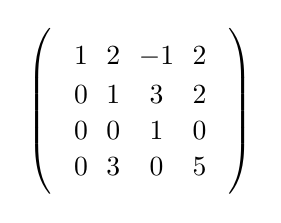
\begin{tikzpicture}
\matrix (m)[matrix of math nodes,left delimiter=(,right delimiter=)]
{
1 & 2 & -1 & 2\\
0 & 1 & 3 & 2\\
0 & 0 & 1 & 0\\
0 & 3 & 0 & 5\\
}; % punto y coma!
% Iluminar de submatriz y elementos
\begin{pgfonlayer}{wfondo}
% Iluminar submatriz desde m_{2,2} hasta m_{4,4}
\iluminar[green!30]{m-2-2}{m-4-4}
%Iluminar elementos de una lista
\foreach \element in {m-4-1,m-3-2,m-2-3,m-1-4}{
\iluminar[violet!30]{\element}{\element} }
% Ilumnar elemento m_{1,1}
\iluminar[gray!30]{m-1-1}{m-1-1}
\end{pgfonlayer}
,\end{tikzpicture}
\end{center}
\end{document}
